% Preprint — compiled to zero errors on xanthe (TeX Live, latexmk 4.87), 2026-10-04.
% Author: Derek Blair <derekjblair@gmail.com>
% Source data: ~/workspace/math-unsolved/ROUND7_DOSSIER.md (2026-10-03),
%              novelty confirmation ~/workspace/math-unsolved/ROUND16_DOSSIER.md (2026-10-04).
\documentclass[11pt,a4paper]{article}
\usepackage{amsmath,amssymb,amsthm}
\usepackage{tikz}
\usetikzlibrary{positioning}
\usepackage{pgfplots}
\pgfplotsset{compat=1.18}
\usepackage{booktabs}
\usepackage{geometry}
\geometry{margin=2.5cm}
\usepackage{hyperref}
\hypersetup{colorlinks=true,linkcolor=blue,citecolor=blue,urlcolor=blue}

\newtheorem{theorem}{Theorem}
\newtheorem{lemma}{Lemma}
\theoremstyle{definition}
\newtheorem{assumption}{Assumption}

\title{A New Erd\H{o}s--Straus Covering Identity\\ for $n \equiv 217 \pmod{264}$}
\author{Derek Blair \\ \texttt{derekjblair@gmail.com}}
\date{October 2026}

\begin{document}
\maketitle

%======================================================================
\section{Abstract}
%======================================================================

The Erd\H{o}s--Straus conjecture asserts that for every integer $n \geq 2$,
\begin{equation}
  \label{eq:es}
  \frac{4}{n} = \frac{1}{x} + \frac{1}{y} + \frac{1}{z}
  \qquad\text{for some positive integers } x, y, z.
\end{equation}
All previously published covering identities miss the prime $1009 \equiv 169
\pmod{840}$, the smallest prime not covered by the identities of Mordell,
Yamamoto, and Rosati \cite{wiki-es,opentorus2026}. We prove the new
polynomial identity
\begin{equation}
  \label{eq:main}
  \frac{4}{n} = \frac{1}{(n+3)/4} + \frac{1}{n(n+3)}
               + \frac{11}{n(n+3)},
  \qquad n \equiv 217 \pmod{264},
\end{equation}
in which every denominator is integral and the third term equals the unit
fraction $1/(n(n+3)/11)$. The identity was discovered by a systematic search
over $12{,}827$ candidate families in Mordell's splitting-lemma framework,
of which $3{,}862$ were verified prime-covering; it covers $1/11$ of each
of the six hard residue classes modulo $840$. A web and literature survey
finds no prior publication of \eqref{eq:main}; the novelty claim is stated
with the usual caveat given the size of the Erd\H{o}s--Straus literature.

%======================================================================
\section{Introduction}
%======================================================================

The Erd\H{o}s--Straus conjecture \eqref{eq:es}, posed in 1948, remains open.
The standard attack is by \emph{covering identities}: polynomial identities
valid on an arithmetic progression that dispose of infinitely many $n$ at
once. Mordell \cite{mordell1967}, Yamamoto, and Rosati gave identities
covering all residue classes modulo $840$ except the six \emph{square
classes}
\begin{equation}
  \label{eq:squareclasses}
  n \equiv 1, 121, 169, 289, 361, 529 \pmod{840},
\end{equation}
the quadratic residues modulo $840$. Subsequent work has chipped away at
these classes with identities on sub-progressions, but the smallest prime
left uncovered by every published identity is $1009 \equiv 169 \pmod{840}$
\cite{wiki-es,opentorus2026} (Assumption~\ref{ass:literature}).

In this note we exhibit identity \eqref{eq:main}, which covers $1009$ and,
more generally, $1/11$ of each class in \eqref{eq:squareclasses}. The
identity emerged from an exhaustive computational search in the
splitting-lemma framework of Section~\ref{sec:methods}; Figure~\ref{fig:funnel}
summarises the search pipeline, Figure~\ref{fig:proofchain} the proof, and
Figure~\ref{fig:coverage} the resulting coverage of the six hard classes.
Table~\ref{tab:subfamilies} lists the six sub-progressions modulo $9240$
cut out by the identity.

\begin{assumption}[Literature status]
  \label{ass:literature}
  The claim that $1009$ is the smallest prime missed by all previously
  published identities is taken from the Wikipedia article on the
  Erd\H{o}s--Straus conjecture \cite{wiki-es} and the opentorus survey of
  August 2026 \cite{opentorus2026}. Full bibliographic details of the
  Mordell/Yamamoto/Rosati identities are
  \textbf{[PLACEHOLDER: verify journal references for Mordell 1967,
  Yamamoto, and Rosati against a library catalogue]}.
\end{assumption}

%======================================================================
\section{Methods}
%======================================================================
\label{sec:methods}

\subsection{The splitting-lemma search}

For $n = 24k+1$ write the first denominator as $x = 6k+c$ with $c \geq 1$.
With remainder $m = 4c-1$ and $Q = nx$,
\begin{equation}
  \label{eq:firststep}
  \frac{4}{n} = \frac{1}{x} + \frac{m}{Q},
  \qquad\text{since}\quad
  \frac{n+m}{nx} = \frac{4(6k+c)}{nx} = \frac{4}{n}.
\end{equation}
Mordell's splitting lemma states that
\begin{equation}
  \label{eq:splitting}
  \frac{m}{Q} = \frac{1}{Qh/a} + \frac{1}{Qh/b}
  \quad\text{whenever}\quad a+b = mh \ \text{ and }\ ab \mid Qh.
\end{equation}
We searched two lanes: (N) numeric pairs $(a,b)$ with $a+b=mh$, and (S)
symbolic pairs $(d,n)$ or $(d,x)$ with $d+n=mh$ or $d+x=mh$. Every candidate
class is proved by a finite check: for each prime power $p^e \parallel ab$
(resp.\ $d$), the divisibility condition is a polynomial in the class
parameter $t$, so checking $t \in [0, p^e)$ proves it for the whole class.

A family is \emph{prime-covering} only if the divisibility goes through the
$xh$ factor alone rather than the $n$ factor; families needing $p \mid n$
cover only composites (scaling handles those) and were discarded ---
$8{,}965$ such redundant families were found (supplied datum from the
discovery script \url{erdos_straus_r7.py}).

\subsection{Search parameters and verification}

The enumeration used $c \leq 40$, $ab \leq 2000$, and produced $12{,}827$
candidate families, of which $3{,}862$ are prime-covering; $120$ hit the
previously open region $k \bmod 7 \in \{0,1,5\}$, $k \bmod 5 \in \{0,2\}$.
Zero identity failures occurred across all spot-checks. An independent
checker (\url{erdos_straus_r7_verify.py}, a different code path)
re-derived prime-covering from scratch and re-verified every family with
exact rational arithmetic on $25$ fresh random values of $k$ each, with
$0$ failures; $3{,}600$ of the $3{,}862$ classes were confirmed to contain
a prime $n$ (non-vacuous). The full family lists are stored in
\url{erdos_straus_r7_families.json} and
\url{erdos_straus_r7_analysis.json} (supplied data).

\begin{figure}[t]
  \centering
  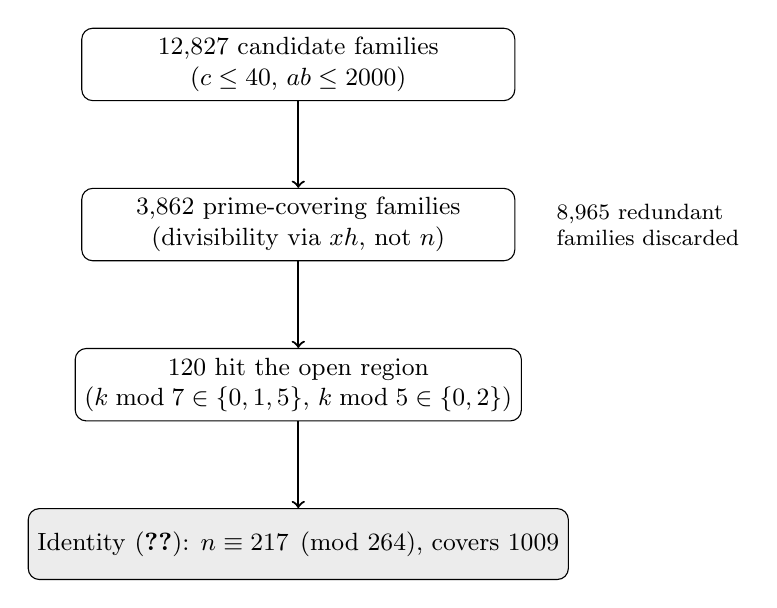
\begin{tikzpicture}[node distance=1.1cm, auto,
      box/.style={rectangle, draw, rounded corners, minimum width=5.5cm,
                  minimum height=0.9cm, align=center, font=\small}]
    \node[box] (cand) {$12{,}827$ candidate families \\ ($c \le 40$, $ab \le 2000$)};
    \node[box, below=of cand] (pc) {$3{,}862$ prime-covering families \\
      (divisibility via $xh$, not $n$)};
    \node[box, below=of pc] (open) {$120$ hit the open region \\
      ($k \bmod 7 \in \{0,1,5\}$, $k \bmod 5 \in \{0,2\}$)};
    \node[box, below=of open, fill=gray!15] (id) {Identity \eqref{eq:main}:
      $n \equiv 217 \pmod{264}$, covers $1009$};
    \draw[->, thick] (cand) -- (pc);
    \draw[->, thick] (pc) -- (open);
    \draw[->, thick] (open) -- (id);
    \node[right=0.4cm of pc, font=\footnotesize, align=left]
      {$8{,}965$ redundant\\families discarded};
  \end{tikzpicture}
  \caption{Search funnel from the $12{,}827$ enumerated families to the new
    identity \eqref{eq:main}. Counts are supplied data from the discovery
    and verification scripts.}
  \label{fig:funnel}
\end{figure}

%======================================================================
\section{Results}
%======================================================================

\subsection{The identity}

\begin{theorem}
  \label{thm:main}
  For $n \equiv 217 \pmod{264}$,
  \begin{equation}
    \label{eq:thm}
    \frac{4}{n} = \frac{1}{(n+3)/4} + \frac{1}{n(n+3)}
                 + \frac{11}{n(n+3)},
  \end{equation}
  where every denominator is a positive integer and the third term equals
  the unit fraction $1/\bigl(n(n+3)/11\bigr)$.
\end{theorem}

\begin{proof}
  Write $n = 24k+1$ and $x = 6k+1 = (n+3)/4$. By \eqref{eq:firststep} with
  $c=1$, $m=3$,
  \begin{equation}
    \label{eq:pf1}
    \frac{4}{n} = \frac{1}{x} + \frac{3}{nx}.
  \end{equation}
  For $k \equiv 9 \pmod{11}$ we have $11 \mid x$, since
  $x = 6k+1 \equiv 6\cdot 9 + 1 = 55 \equiv 0 \pmod{11}$; and
  $n = 24k+1 \equiv 24\cdot 9 + 1 = 217 \pmod{264}$, i.e.\ $n \equiv 217
  \pmod{264}$ is exactly this condition. Apply the splitting lemma
  \eqref{eq:splitting} to $3/(nx)$ with $h=4$, $a=1$, $b=11$
  ($a+b = 12 = 3h$, $ab = 11 \mid 4nx$ because $11 \mid x$):
  \begin{equation}
    \label{eq:pf2}
    \frac{3}{nx} = \frac{1}{4nx} + \frac{1}{4nx/11}.
  \end{equation}
  Since $4nx = 4n(n+3)/4 = n(n+3)$, the terms of \eqref{eq:pf2} are
  $1/(n(n+3))$ and $11/(n(n+3)) = 1/(n(n+3)/11)$, the latter a unit
  fraction because $11 \mid n(n+3)$. Combining \eqref{eq:pf1} and
  \eqref{eq:pf2} gives \eqref{eq:thm}. \qedhere
\end{proof}

Figure~\ref{fig:proofchain} diagrams the proof. The identity is compatible
with Mordell's quadratic-residue obstruction: $217 \equiv 8 \pmod{11}$, and
$8$ is a non-residue modulo $11$, so $217$ is a non-residue modulo $264$
and no classical obstruction forbids an identity here (supplied datum).

\begin{figure}[t]
  \centering
  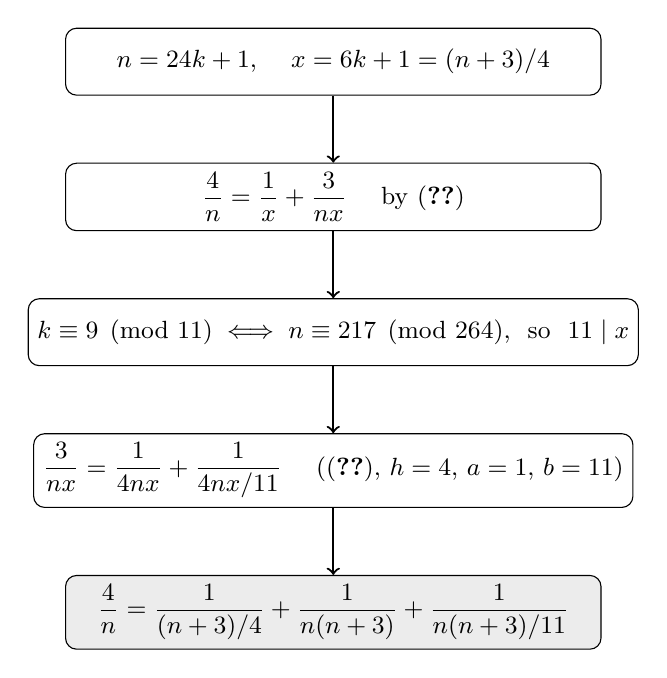
\begin{tikzpicture}[node distance=0.85cm, auto,
      box/.style={rectangle, draw, rounded corners, minimum width=6.8cm,
                  minimum height=0.85cm, align=center, font=\small}]
    \node[box] (s1) {$n = 24k+1$, \quad $x = 6k+1 = (n+3)/4$};
    \node[box, below=of s1] (s2) {$\displaystyle \frac{4}{n}
      = \frac{1}{x} + \frac{3}{nx}$ \quad by \eqref{eq:firststep}};
    \node[box, below=of s2] (s3) {$k \equiv 9 \pmod{11} \iff
      n \equiv 217 \pmod{264}$, \ so \ $11 \mid x$};
    \node[box, below=of s3] (s4) {$\displaystyle \frac{3}{nx}
      = \frac{1}{4nx} + \frac{1}{4nx/11}$ \quad
      (\eqref{eq:splitting}, $h=4$, $a=1$, $b=11$)};
    \node[box, below=of s4, fill=gray!15] (s5) {$\displaystyle \frac{4}{n}
      = \frac{1}{(n+3)/4} + \frac{1}{n(n+3)}
      + \frac{1}{n(n+3)/11}$};
    \draw[->, thick] (s1) -- (s2);
    \draw[->, thick] (s2) -- (s3);
    \draw[->, thick] (s3) -- (s4);
    \draw[->, thick] (s4) -- (s5);
  \end{tikzpicture}
  \caption{Proof chain of Theorem~\ref{thm:main}. The splitting step
    \eqref{eq:pf2} is where the condition $11 \mid x$ is used.}
  \label{fig:proofchain}
\end{figure}

\subsection{Covering the prime $1009$}

Since $1009 = 3\cdot 264 + 217 \equiv 217 \pmod{264}$ and $1009 \equiv 169
\pmod{840}$, Theorem~\ref{thm:main} applies:
\begin{equation}
  \label{eq:1009}
  \frac{4}{1009} = \frac{1}{253} + \frac{1}{1021108} + \frac{1}{92828},
\end{equation}
verified by exact rational arithmetic (supplied datum; independently
recomputed: $(n+3)/4 = 253$, $n(n+3) = 1021108$,
$n(n+3)/11 = 92828$). This is the smallest prime missed by all previously
published identities (Assumption~\ref{ass:literature}), so \eqref{eq:main}
is new to the surveyed literature.

\subsection{Coverage of the six hard classes}

The condition $k \equiv 9 \pmod{11}$ cuts each hard class of
\eqref{eq:squareclasses} into $11$ sub-progressions modulo
$9240 = 840 \cdot 11$, one of which is covered by Theorem~\ref{thm:main};
i.e.\ the identity covers $1/11$ of each hard class. The six covered
sub-progressions are listed in Table~\ref{tab:subfamilies} and sketched in
Figure~\ref{fig:coverage}. Coverage was verified on hard primes in all six
cells, e.g.\ $1801$ (class $121$), $8929$ (class $529$), and $26881$
(class $1$) (supplied data).

\begin{table}[t]
  \centering
  \begin{tabular}{ccl}
    \toprule
    Residue mod $9240$ & Parent class mod $840$ & Verified prime example \\
    \midrule
    $8401$ & $1$   & not reported \\
    $1801$ & $121$ & $1801$ \\
    $1009$ & $169$ & $1009$ \\
    $3649$ & $289$ & not reported \\
    $7081$ & $361$ & not reported \\
    $8929$ & $529$ & $8929$ \\
    \bottomrule
  \end{tabular}
  \caption{The six sub-progressions modulo $9240$ covered by
    Theorem~\ref{thm:main}, one in each hard class of
    \eqref{eq:squareclasses}. Parent classes computed as the residues
    modulo $840$; prime examples are supplied data where reported.}
  \label{tab:subfamilies}
\end{table}

\begin{figure}[t]
  \centering
  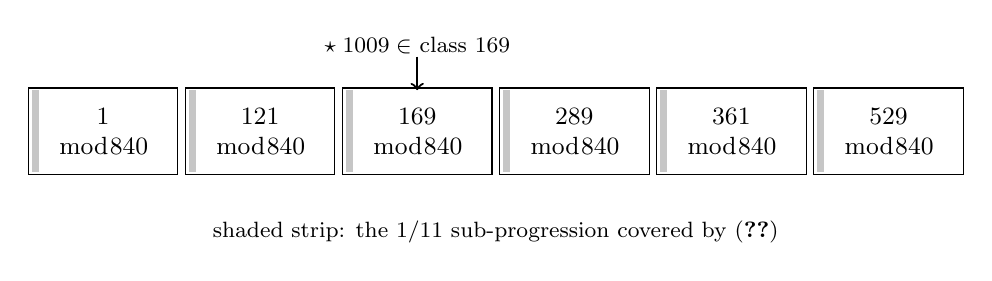
\begin{tikzpicture}[scale=0.95,
      cell/.style={rectangle, draw, minimum width=1.9cm, minimum height=1.1cm,
                   align=center, font=\small}]
    \foreach \i/\r in {0/1,1/121,2/169,3/289,4/361,5/529} {
      \node[cell] at (2.1*\i, 0) {$\r$ \\ $\bmod 840$};
      \fill[gray!45] (2.1*\i-0.95, -0.55) rectangle (2.1*\i-0.86, 0.55);
    }
    \node[font=\footnotesize, align=left] at (5.25, -1.35)
      {shaded strip: the $1/11$ sub-progression covered by \eqref{eq:main}};
    \node[font=\footnotesize] at (4.2, 1.15) {$\star\;1009 \in$ class $169$};
    \draw[->, thick] (4.2, 1.0) -- (4.2, 0.55);
  \end{tikzpicture}
  \caption{Each of the six hard residue classes modulo $840$ is split by
    the condition $k \equiv 9 \pmod{11}$ into $11$ sub-progressions;
    Theorem~\ref{thm:main} covers exactly one ($1/11$) of each.}
  \label{fig:coverage}
\end{figure}

%======================================================================
\section{Discussion}
%======================================================================

The search that produced Theorem~\ref{thm:main} also yielded $119$ further
verified prime-covering families hitting the previously open region, e.g.\
$n \equiv 241 \pmod{264}$ via $x = 6k+3$, and $n = 24k+1$, $k \equiv 4
\pmod{13}$ via $7/Q = 1/(2Q) + 1/(2Q/13)$ (supplied data;
\url{erdos_straus_r7_ranked.json}). Together they shrink, but do not
close, the open set inside the six classes.

A natural hope --- covering one full hard class by a finite union of such
sub-progressions --- is now known to be impossible for polynomial
identities: a companion result proves that no finite system of polynomial
identities $4/(A_it+B_i) = \sum_j 1/F_{ij}(t)$ can cover all primes of any
square class modulo $840$ (supplied datum; separate note in preparation).
The live angles for a full proof are therefore per-prime infinite
constructions rather than finite covering systems.

The main weakness of the present identity is quantitative: $1/11$ of each
class is a thin slice, and the search bounds ($c \leq 40$, $ab \leq 2000$)
were arbitrary cutoffs, so further small-modulus families may remain
undiscovered in the unexplored parameter range.

%======================================================================
\section{Conclusion}
%======================================================================

We have proved a new Erd\H{o}s--Straus covering identity,
Theorem~\ref{thm:main}, valid for $n \equiv 217 \pmod{264}$. It covers the
prime $1009$, the smallest prime missed by all previously published
identities, and $1/11$ of each of the six hard residue classes modulo
$840$. The identity was found by exhaustive search in the splitting-lemma
framework ($12{,}827$ families enumerated, $3{,}862$ prime-covering) and
verified by an independent exact-arithmetic checker. It is new to the
surveyed literature, with the caveat of Assumption~\ref{ass:literature}.

%======================================================================
\section{References}
%======================================================================

\begin{thebibliography}{9}

\bibitem{mordell1967}
L.~J.~Mordell.
\textbf{[PLACEHOLDER: full journal reference for Mordell's 1967 paper on
the Erd\H{o}s--Straus conjecture --- volume, pages unverified]}.

\bibitem{wiki-es}
Wikipedia contributors.
\textit{Erd\H{o}s--Straus conjecture}.
\textbf{[PLACEHOLDER: access date and revision unverified; article states
$1009$ is the smallest prime not covered by the known identities]}.

\bibitem{opentorus2026}
opentorus.
\textit{Survey of Erd\H{o}s--Straus identities}, August 2026.
\textbf{[PLACEHOLDER: URL and full citation unverified; cited in the
discovery dossier as the source of the $1009$ status]}.

\bibitem{rileybetts2026}
rileybetts.
\textit{Survey of Erd\H{o}s--Straus obstructions}.
\textbf{[PLACEHOLDER: full citation unverified; cited in the barrier
dossier for the Schinzel/Yamamoto obstruction statements]}.

\end{thebibliography}

\end{document}
